%-------------------------------------------------------------------------
\begin{figure}[t]
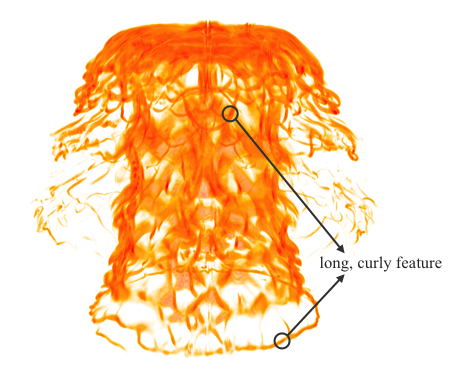
\includegraphics[width=0.9\linewidth]{combustion_labeled.png}
\caption{The volume rendering of a single time step of the combustion data set.}
\label{fig:combustion-labeled}
\end{figure}
%-------------------------------------------------------------------------

\section{Results}

We first test our feature extraction and tracking algorithm on a $256\times256\times256$ vortex data set obtained from a combustion solver that can simulate turbulent flames. In this data set, each voxel contains the magnitude value of vorticity derived from velocity using a curl operator. As time evolves, vortical features may vary from small amassed blob features to long curly features that span over large portion of the volume, as shown in Figure~\ref{fig:combustion-labeled}.

%\subsection{Performance Result}

The volume data can be generated either in advance or on the fly, and thus we ignore the I/O cost and only focus on the computation time for the following three portions.

\textbf{Time for extracting features ($T_{extract}$).}
%
Since we use the region-growing based algorithm to extract features, given a fix specification of features, the computation time is mainly determined by the size of the volume as well as the number of processors being used. Once the raw volume data and its partitioning, a.k.a. the size of each data block is determined, the computation time for extracting residing features remains approximately the same. In post-processing, the size of each data block decreases with the increasing number, and hence so does the time spent on extracting features. As depicted in Figure~\ref{fig:feature-extraction}, $T_{extract}$ is approximately log-linear decreased as the number of processors grows from 8 to 16384.

\begin{figure}[t]
\centering
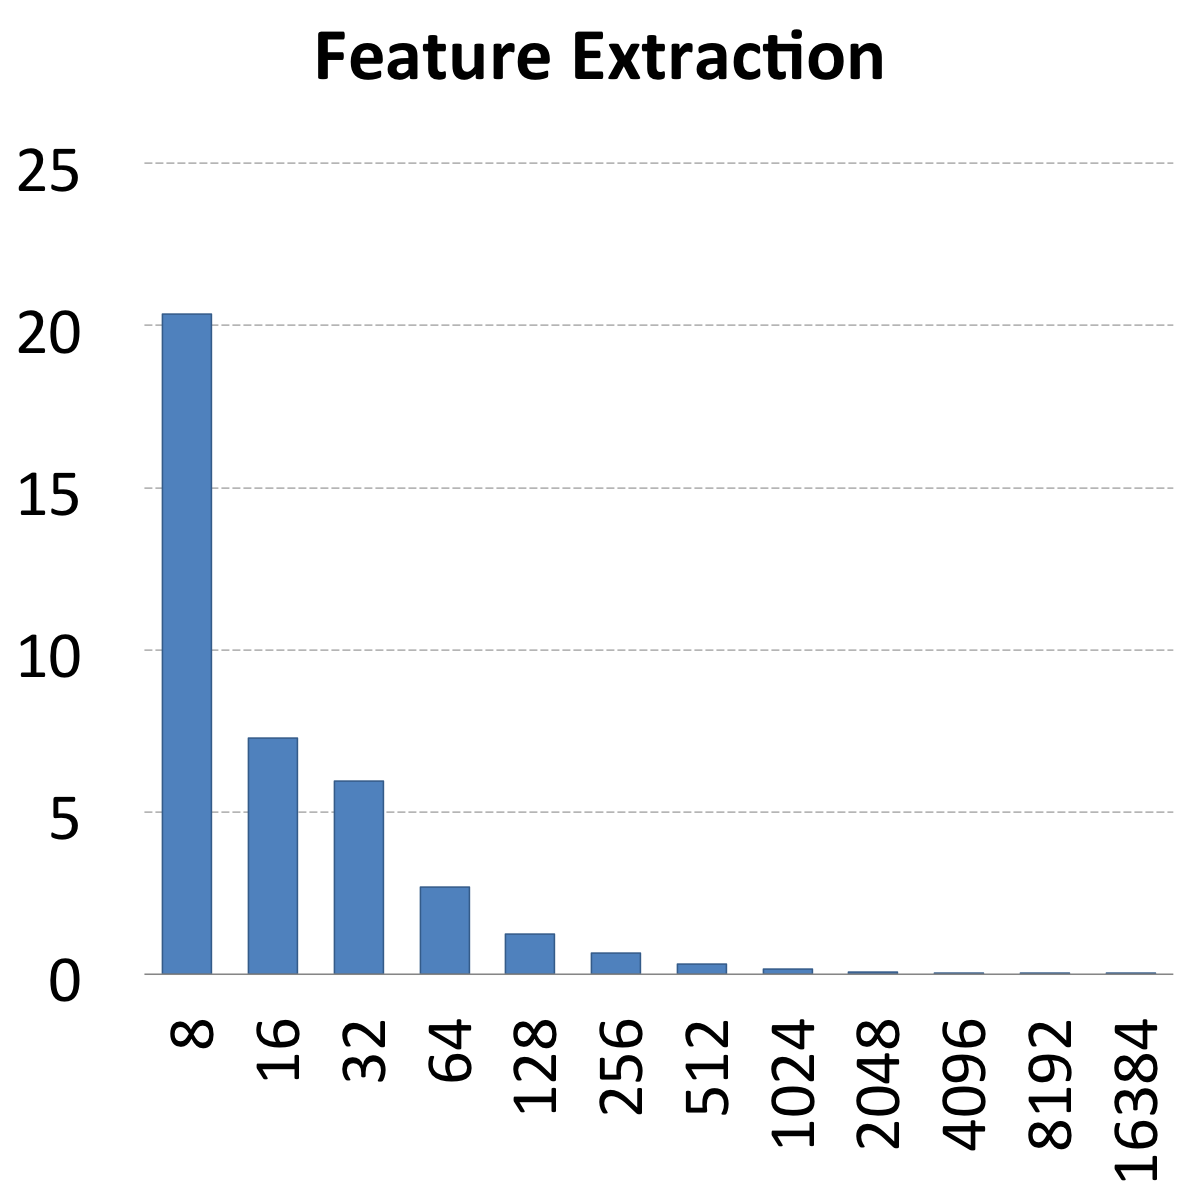
\includegraphics[width=1.0\linewidth]{feature_extraction.png}\\
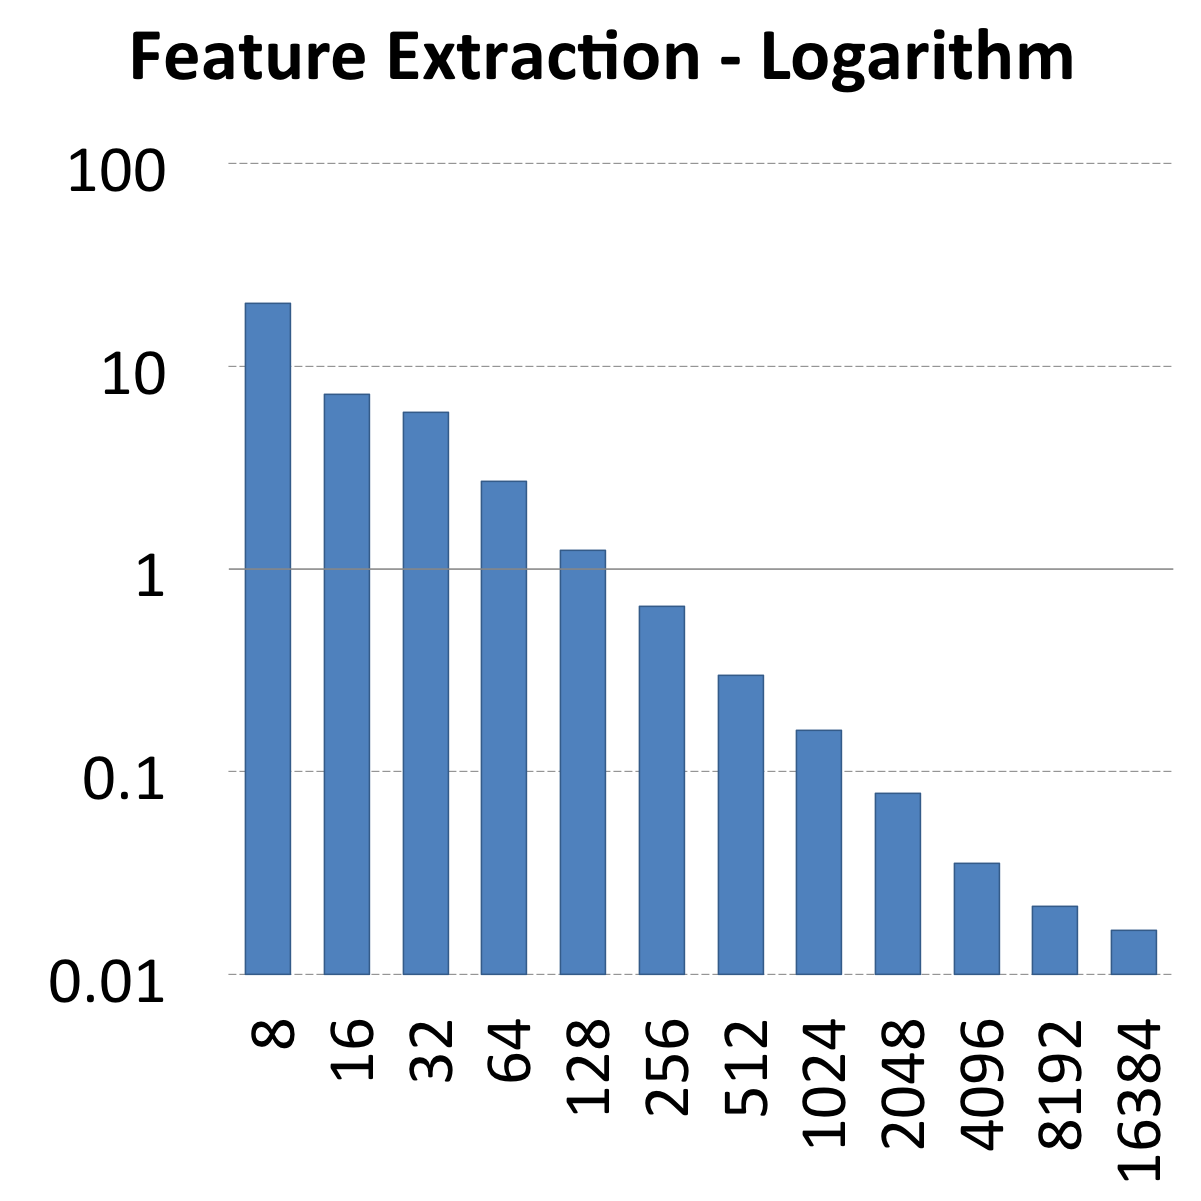
\includegraphics[width=1.0\linewidth]{feature_extraction_log.png}
\caption{Computation time for feature extraction. The top plot is shown in linear scale, and the bottom plot is shown in logarithmic scale. It is linearly scalable as the number of processor increases}
\label{fig:feature-extraction}
\end{figure}

\textbf{Create Local Connectivity Tree ($T_{create}$)}
%
Despite the size of each data block, the computation cost for creating and updating local connectivity tree is dependent on the number of the features extracted within the original volume, or more precisely, the number of features that touches the boundary surface of their residing data block. As shown in Figure~\ref{fig:create-local-graph}, similar to $T_{extract}$, $T_{create}$ decreases as the number of processors increases in post-processing, as the the number of feature-on-boundary decreases accordingly. For the combustion data set, it takes an average of 0.1 seconds to create the local connectivity tree, approximately 0.5\% the time of $T_{extract}$ using the same amount of processors. This portion increases but does not succeed 1\% in out test, hence $T_{create}$ is not considered as a bottleneck. %\textcolor{red}{for in-situ visualization however... }

\begin{figure}[t]
\centering
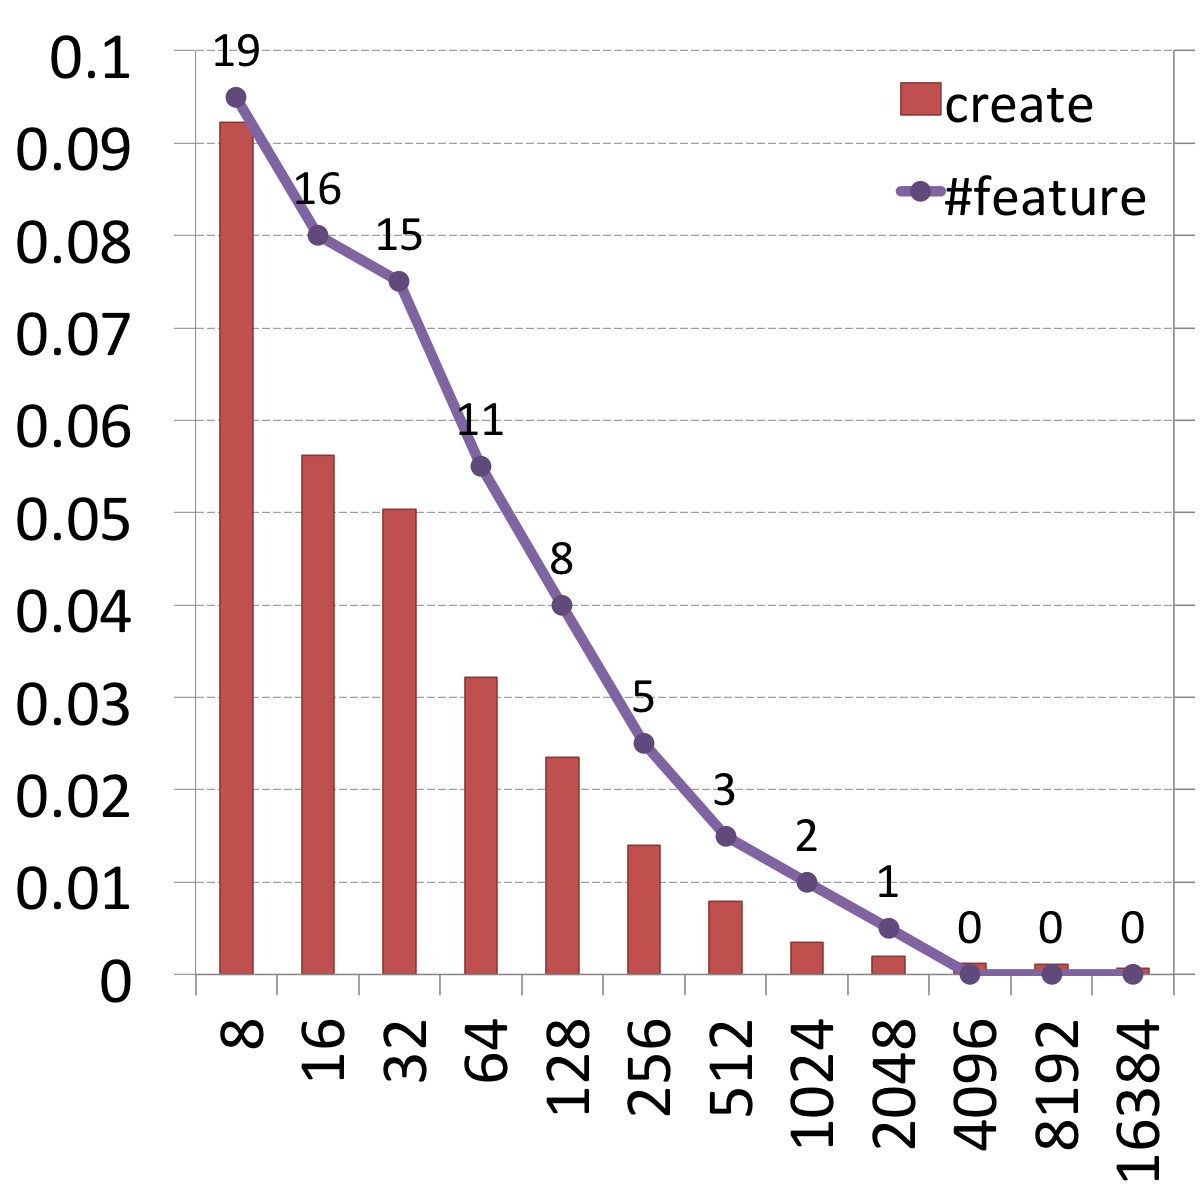
\includegraphics[width=1.0\linewidth]{create_local_graph.png}
%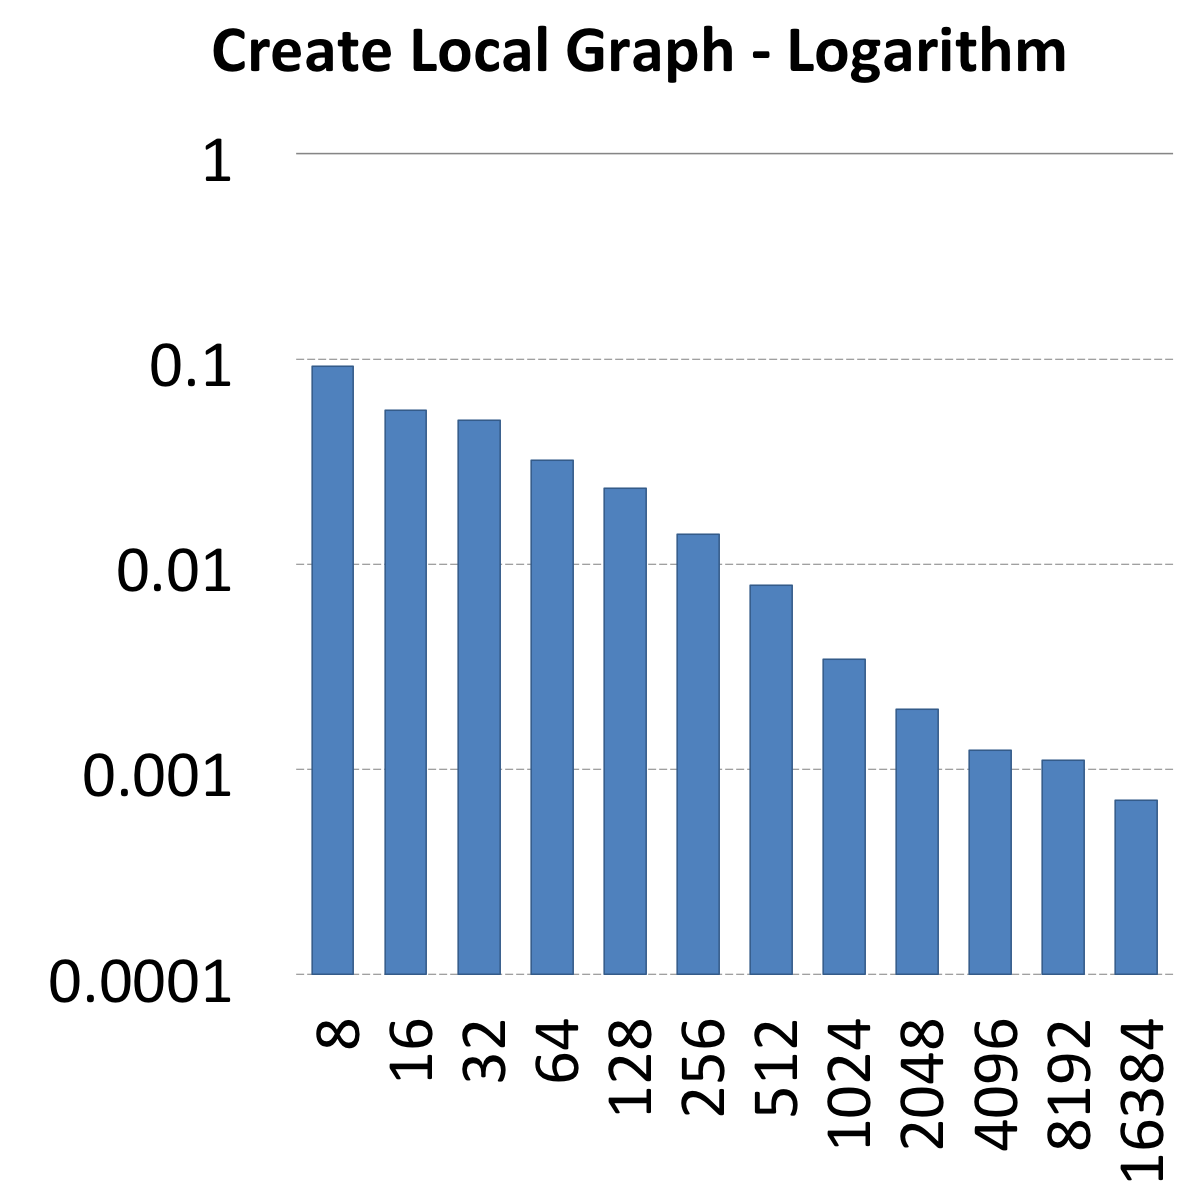
\includegraphics[width=0.6\linewidth]{create_local_graph_log.png}
\caption{Computation time for creating local connectivity tree. It is linearly scalable as the number of processor increases. The time is approximately proportional to the number of features-on-boundary. Note that, for the processor numbers greater than 4096, the average feature numbers are between 0 and 0.5 and are rounded to 0.}
\label{fig:create-local-graph}
\end{figure}

\textbf{Create Global Connectivity Information ($T_{merge}$)}
%
We also test the centralized approach and the decentralized approach in creating global connectivity information that is the major factor related to the scalability of our algorithm. Though the number of features-on-boundary decreases as more processors involved, the communication time for the centralized approach increases as $N_p$ increases. According to the comparison depicted in Figure~\ref{fig:local-vs-global}, we can see that the centralized approach is suitable for the scenarios that we only need a small number of processors, and the decentralized approach for creating connectivity information using a relatively large amount of the processors.

\begin{figure}[ht]
\centering
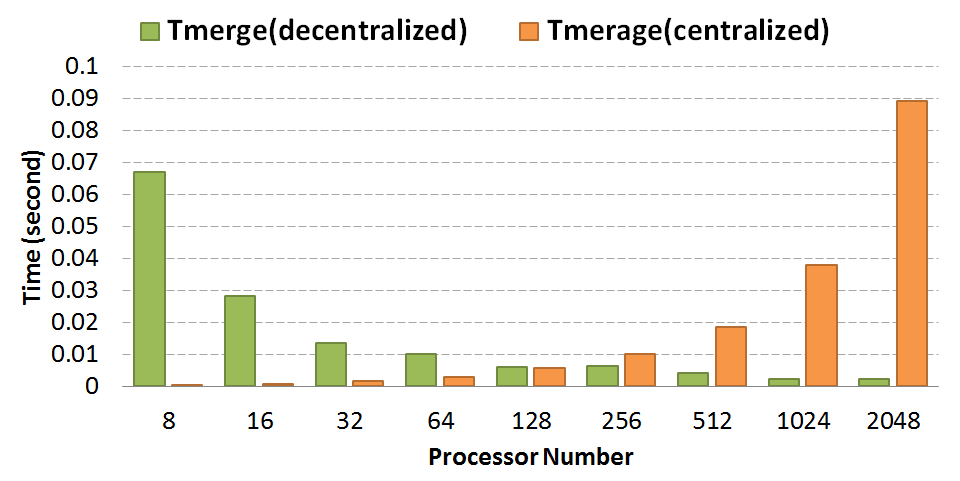
\includegraphics[width=1.0\linewidth]{local_vs_global.png}
\caption{The comparison between the computation time for the centralized approach and the decentralized approach. The centralized approach works well for a small number of processors while the decentralized approach exceeds after a certain number, 128 processors for the combustion data set, is used.}
\label{fig:local-vs-global}
\end{figure}

As shown in Figure~\ref{fig:global-merge}, the total time $T_{merge}$ for the centralized approach exceeds $T_{extract}$ after certain amount of processors, 2048, for the combustion data set, which makes the overall execution time rebounds . On the other hand, the decentralized approach  scales well up to 16384 processors for the combustion data set, as the communication cost is as low as ${O(\sqrt[3]{N_p})}$.

\begin{figure}[t]
\centering
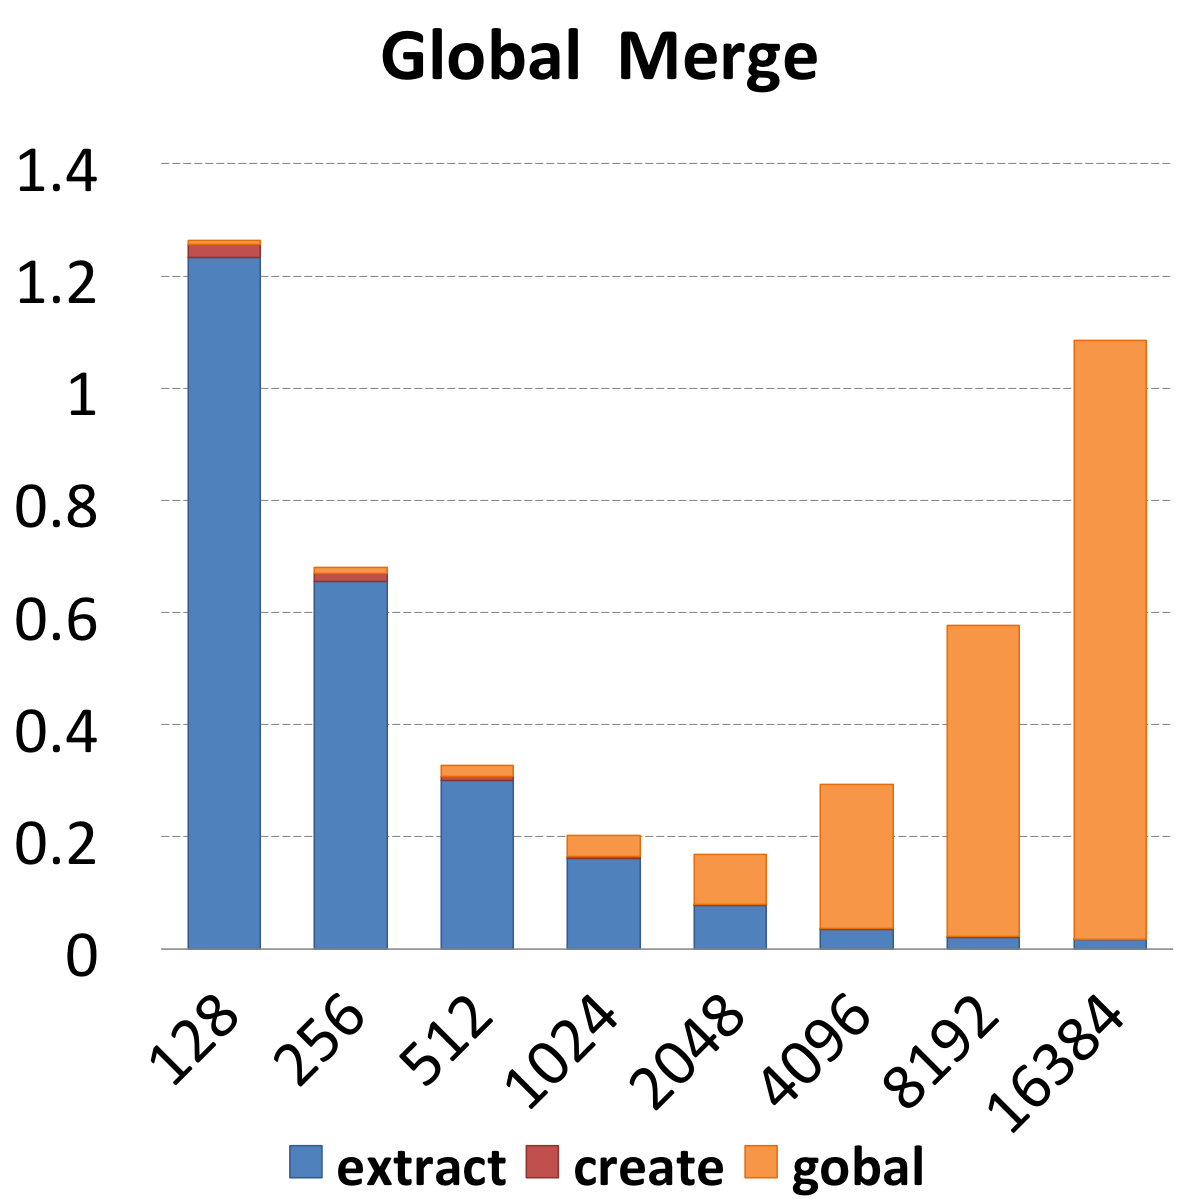
\includegraphics[width=1.0\linewidth]{global_merge.png}\\
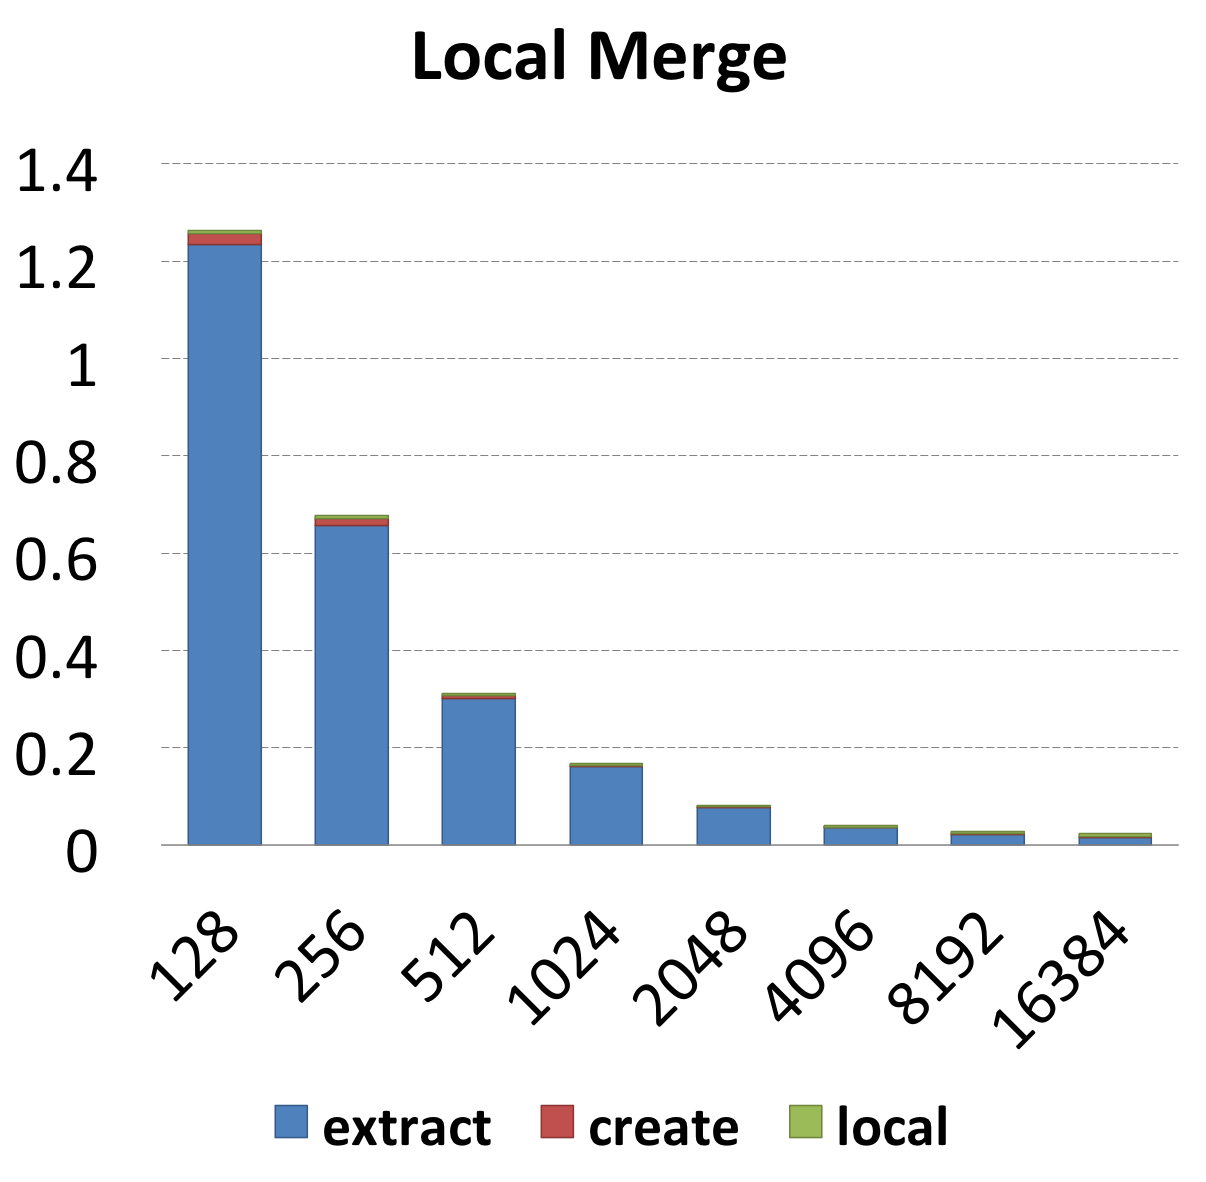
\includegraphics[width=1.0\linewidth]{local_merge.png}
\caption{Total computation time comparison for different merging strategy. The decentralized-global-merge strategy scaled up to 2048 processors but the merging time outweighs the extraction time when using more processors; The decentralized-local-merge strategy scaled log-linearly up 16384 processors for the combustion data set.}
\label{fig:global-merge}
\end{figure}


